

\subsection{Perfilador en Laboratorio 7}
\begin{frame}{Perfilador en Laboratorio 7}
    \begin{onlyenv}<1>
        
    
    Primera iteración mecánica
    \begin{columns}[c]
        \begin{column}{0.4\textwidth}
            \begin{itemize}
                \item Soporte adosable a la mesa óptica por perros. Facil colocación
                \item Motor encastrado en soporte. No hay artefactos mecánicos
                \item Tambor de metal con superficie no reflectante
                \item No permite medir fácilmente en el otro eje. Habrá otra iteración
            \end{itemize}
        \end{column}
        \begin{column}{0.5\textwidth}
            \begin{figure}
                \centering
                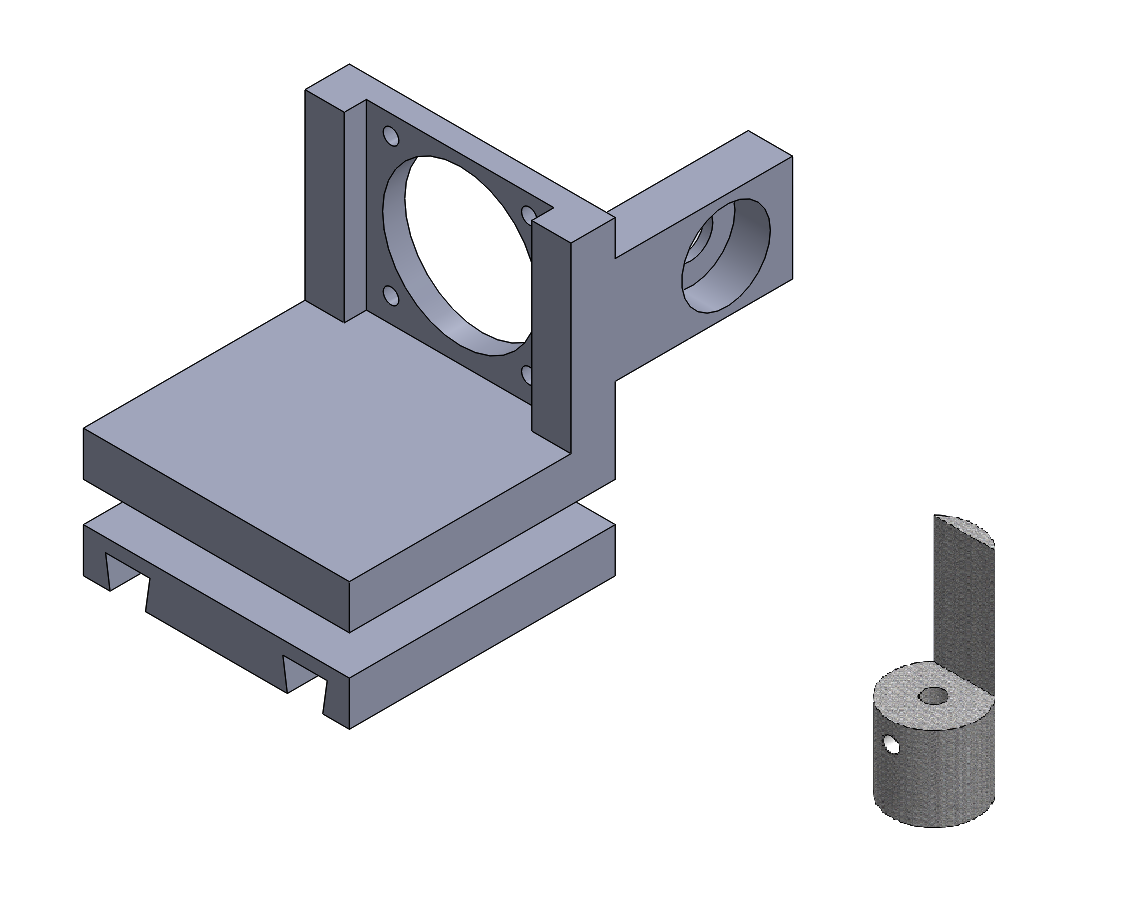
\includegraphics[width=\textwidth]{fig/perfilador/soporte_labo7_1}
             
                \label{fig:soporte_labo7}
            \end{figure}
        \end{column}
    \end{columns}
    \end{onlyenv}
    \begin{onlyenv}<2>
        
    Segunda iteración mecánica.
    \begin{columns}[c]
        \begin{column}{0.4\textwidth}
            \begin{figure}
                \centering
                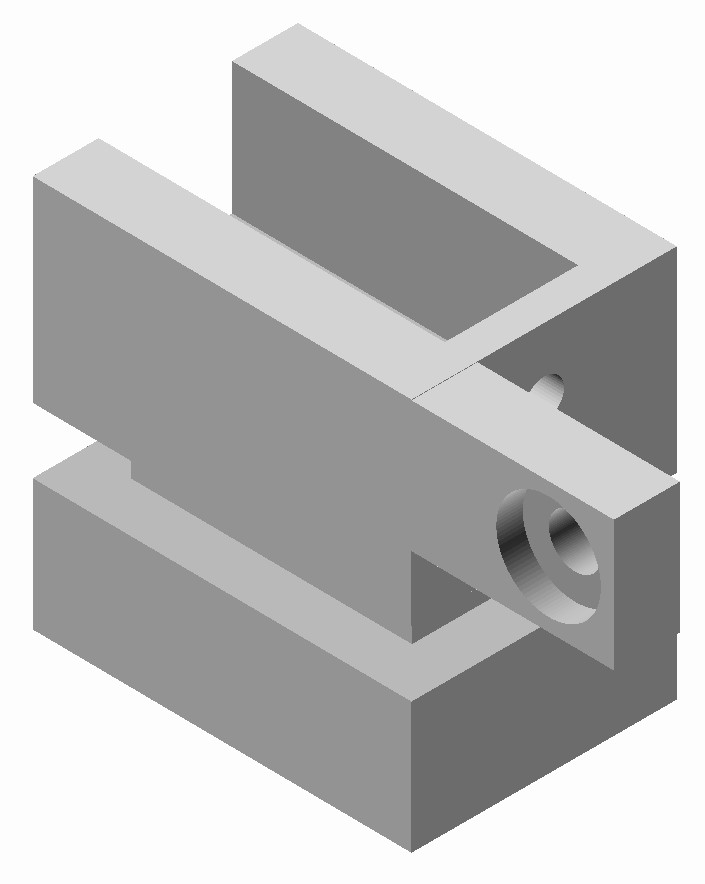
\includegraphics[width=0.8\textwidth]{fig/perfilador/soporte_labo7_2}
             
                \label{fig:soporte_labo7}
            \end{figure}
        \end{column}
        \begin{column}{0.5\textwidth}
            \begin{itemize}
                \item  Motor NEMA 8, reduce un 500\% el tamaño.
                \item  Soporte fácil de colocar sobre la mesa óptica y sobre un soporte en altura
                \item  Tambor reimpreso en plástico
            \end{itemize}
            
        \end{column}
    \end{columns}
    \end{onlyenv}
\end{frame}
